\documentclass[a4paper]{beamer}

\usepackage[english]{babel}
\usepackage[utf8]{inputenc}
\usepackage{graphicx}
\usepackage{subcaption}
\usepackage{hyperref}
\usepackage{listings}

%\usepackage{color}
\definecolor{darkgreen}{RGB}{0 100 0}

\definecolor{lightgray}{RGB}{240 240 240}
\newcommand{\code}[1]{\colorbox{lightgray}{\lstinline~#1~}}

\definecolor{light-blue}{RGB}{210,210,255}
\definecolor{light-red}{RGB}{255,210,210}
\definecolor{light-yellow}{RGB}{255, 255, 150}
\definecolor{light-grey}{RGB}{220, 220, 220}

\lstset{language=Java, tabsize=4, literate={ç}{{\c{c}}}1 {é}{{\'e}}1 {è}{{\`e}}1 {ê}{{\^e}}1 {à}{{\`a}}1 {î}{{\^i}}1 {É}{{\'E}}1 {ô}{{\^o}}1, stringstyle=\color{red}, keywordstyle=\color{blue}, identifierstyle=\color{black}, escapeinside={♠}{♣}}

\usetheme{Darmstadt}
\definecolor{clearblueifnti}{RGB}{24,116,220}
\setbeamercolor{title}{use=structure,bg=clearblueifnti,fg=white}



\makeatletter
\setbeamertemplate{title page}{
  \vbox{}
  \vfill
  \begingroup
    \centering\hspace{2cm}
    \begin{minipage}{.7\textwidth}
    \begin{beamercolorbox}[sep=8pt,center,shadow=true,rounded=true]{title}
      \usebeamerfont{title}\inserttitle\par%
      \ifx\insertsubtitle\@empty%
      \else%
        \vskip0.25em%
        {\usebeamerfont{subtitle}\usebeamercolor[fg]{subtitle}\insertsubtitle\par}%
      \fi%     
    \end{beamercolorbox}%
    \end{minipage}

    \vskip2.8em\par
    \begin{minipage}{\textwidth}
    \begin{beamercolorbox}[sep=8pt,center]{author}
      \usebeamerfont{author}\insertauthor
    \end{beamercolorbox}
    \end{minipage}

    \begin{minipage}{\textwidth}
    \begin{beamercolorbox}[sep=8pt,center]{institute}
      \usebeamerfont{institute}\insertinstitute
    \end{beamercolorbox}
    \end{minipage}

    \begin{minipage}{\textwidth}
    \begin{beamercolorbox}[sep=8pt,center]{date}
      \usebeamerfont{date}\insertdate
    \end{beamercolorbox}
    \end{minipage}
    \vskip0.5em
    {\usebeamercolor[fg]{titlegraphic}\inserttitlegraphic\par}
  \endgroup
  \vfill
}
\makeatother

\title{Docker}
\subtitle[DAP]{UE Libre}
\institute{IFNTI L3}
\author{KONDI Abdoul malik \\ ADJANAYO Simone \thanks{Inspiré de la documentation docker et du cours d'openclassroom sur docker}}
\date{\today}

\setbeamertemplate{footline}
{
  \hbox{
  \begin{beamercolorbox}[wd=.3\paperwidth,ht=2.25ex,dp=1ex,center]{author in head/foot}
    \usebeamerfont{author in head/foot}\insertshortauthor
  \end{beamercolorbox}
  \begin{beamercolorbox}[wd=.6\paperwidth,ht=2.25ex,dp=1ex,center]{date in head/foot}
    \usebeamerfont{date in head/foot}\insertshortsubtitle{} : \inserttitle{} - \insertshortinstitute{} - \insertdate
  \end{beamercolorbox}
  \begin{beamercolorbox}[wd=.1\paperwidth,ht=2.25ex,dp=1ex,center]{title in head/foot}
    \usebeamerfont{title in head/foot}\insertframenumber{} / \inserttotalframenumber
  \end{beamercolorbox}}
}

\usebackgroundtemplate{
\includegraphics[width=\paperwidth,height=\paperheight]{CharteGraphiquePresentationCorps_etroit}}

\begin{document}

{
\setbeamertemplate{headline}{\vskip\headheight}
\setbeamertemplate{footline}{}
\usebackgroundtemplate{
\includegraphics[width=\paperwidth,height=\paperheight]{CharteGraphiquePresentationPageDeGarde}}
\begin{frame}[plain]
	%\vspace{5cm}
	\titlepage
\end{frame}
}

\begin{frame}{Table des matières}
	%\begin{multicols}{2}
	\tableofcontents
	%\end{multicols}
\end{frame}

{\AtBeginSection[]{
  \begin{frame}
  \vfill
  \centering
  \begin{beamercolorbox}[sep=8pt,center,shadow=true,rounded=true]{title}
    \usebeamerfont{title}\insertsection\par
  \end{beamercolorbox}
  \vfill
  \end{frame}
}

\section{Concept général}

\begin{frame}{Qu'est ce que docker ?}
\begin{center}

\includegraphics[scale=0.13]{images/docker.png}

\includegraphics[scale=0.8]{images/dotcloud.png}
\end{center}
\begin{block}{Docker}
\begin{itemize}
\item[•] Une plateforme de conteneurisation.
\item[•] Créer en 2013 par la société dotCloud.
\end{itemize}
\end{block}
\end{frame}

\begin{frame}{Objectifs}
\begin{block}{L'objectif de docker}
est faire tourné qu'un seul processus dans un conteneur.
\end{block}
\end{frame}

\begin{frame}{Pourquoi docker ?}
\begin{block}{Raisons}
\begin{itemize}
\item[•] Évité les difficultés lier au déploiement.
\item[•] Avoir un environnement unifié et fonctionnel (pratique lorsque les projets sont en collaboration).
\end{itemize}
\end{block}
\end{frame}

\begin{frame}{Qu'est ce que le déploiement 1/2}
	\begin{block}{Acteurs}
	Les deux principaux acteurs dans un cycle de déploiement sont:
	\begin{itemize}
	\item[•] Les développeurs.
	\item[•] Les administrateurs système.
	\end{itemize}
	\end{block}
	\begin{block}{Exemple d'équation entre ces deux acteurs}
	Administrateur système = Garant de la stabilité de la sécurité des systèmes informatique\\
    Développeurs = Créateurs de nouvelles fonctionnalité et applications
	\end{block}
\end{frame}

\begin{frame}{Cycle de déploiement}
\begin{center}
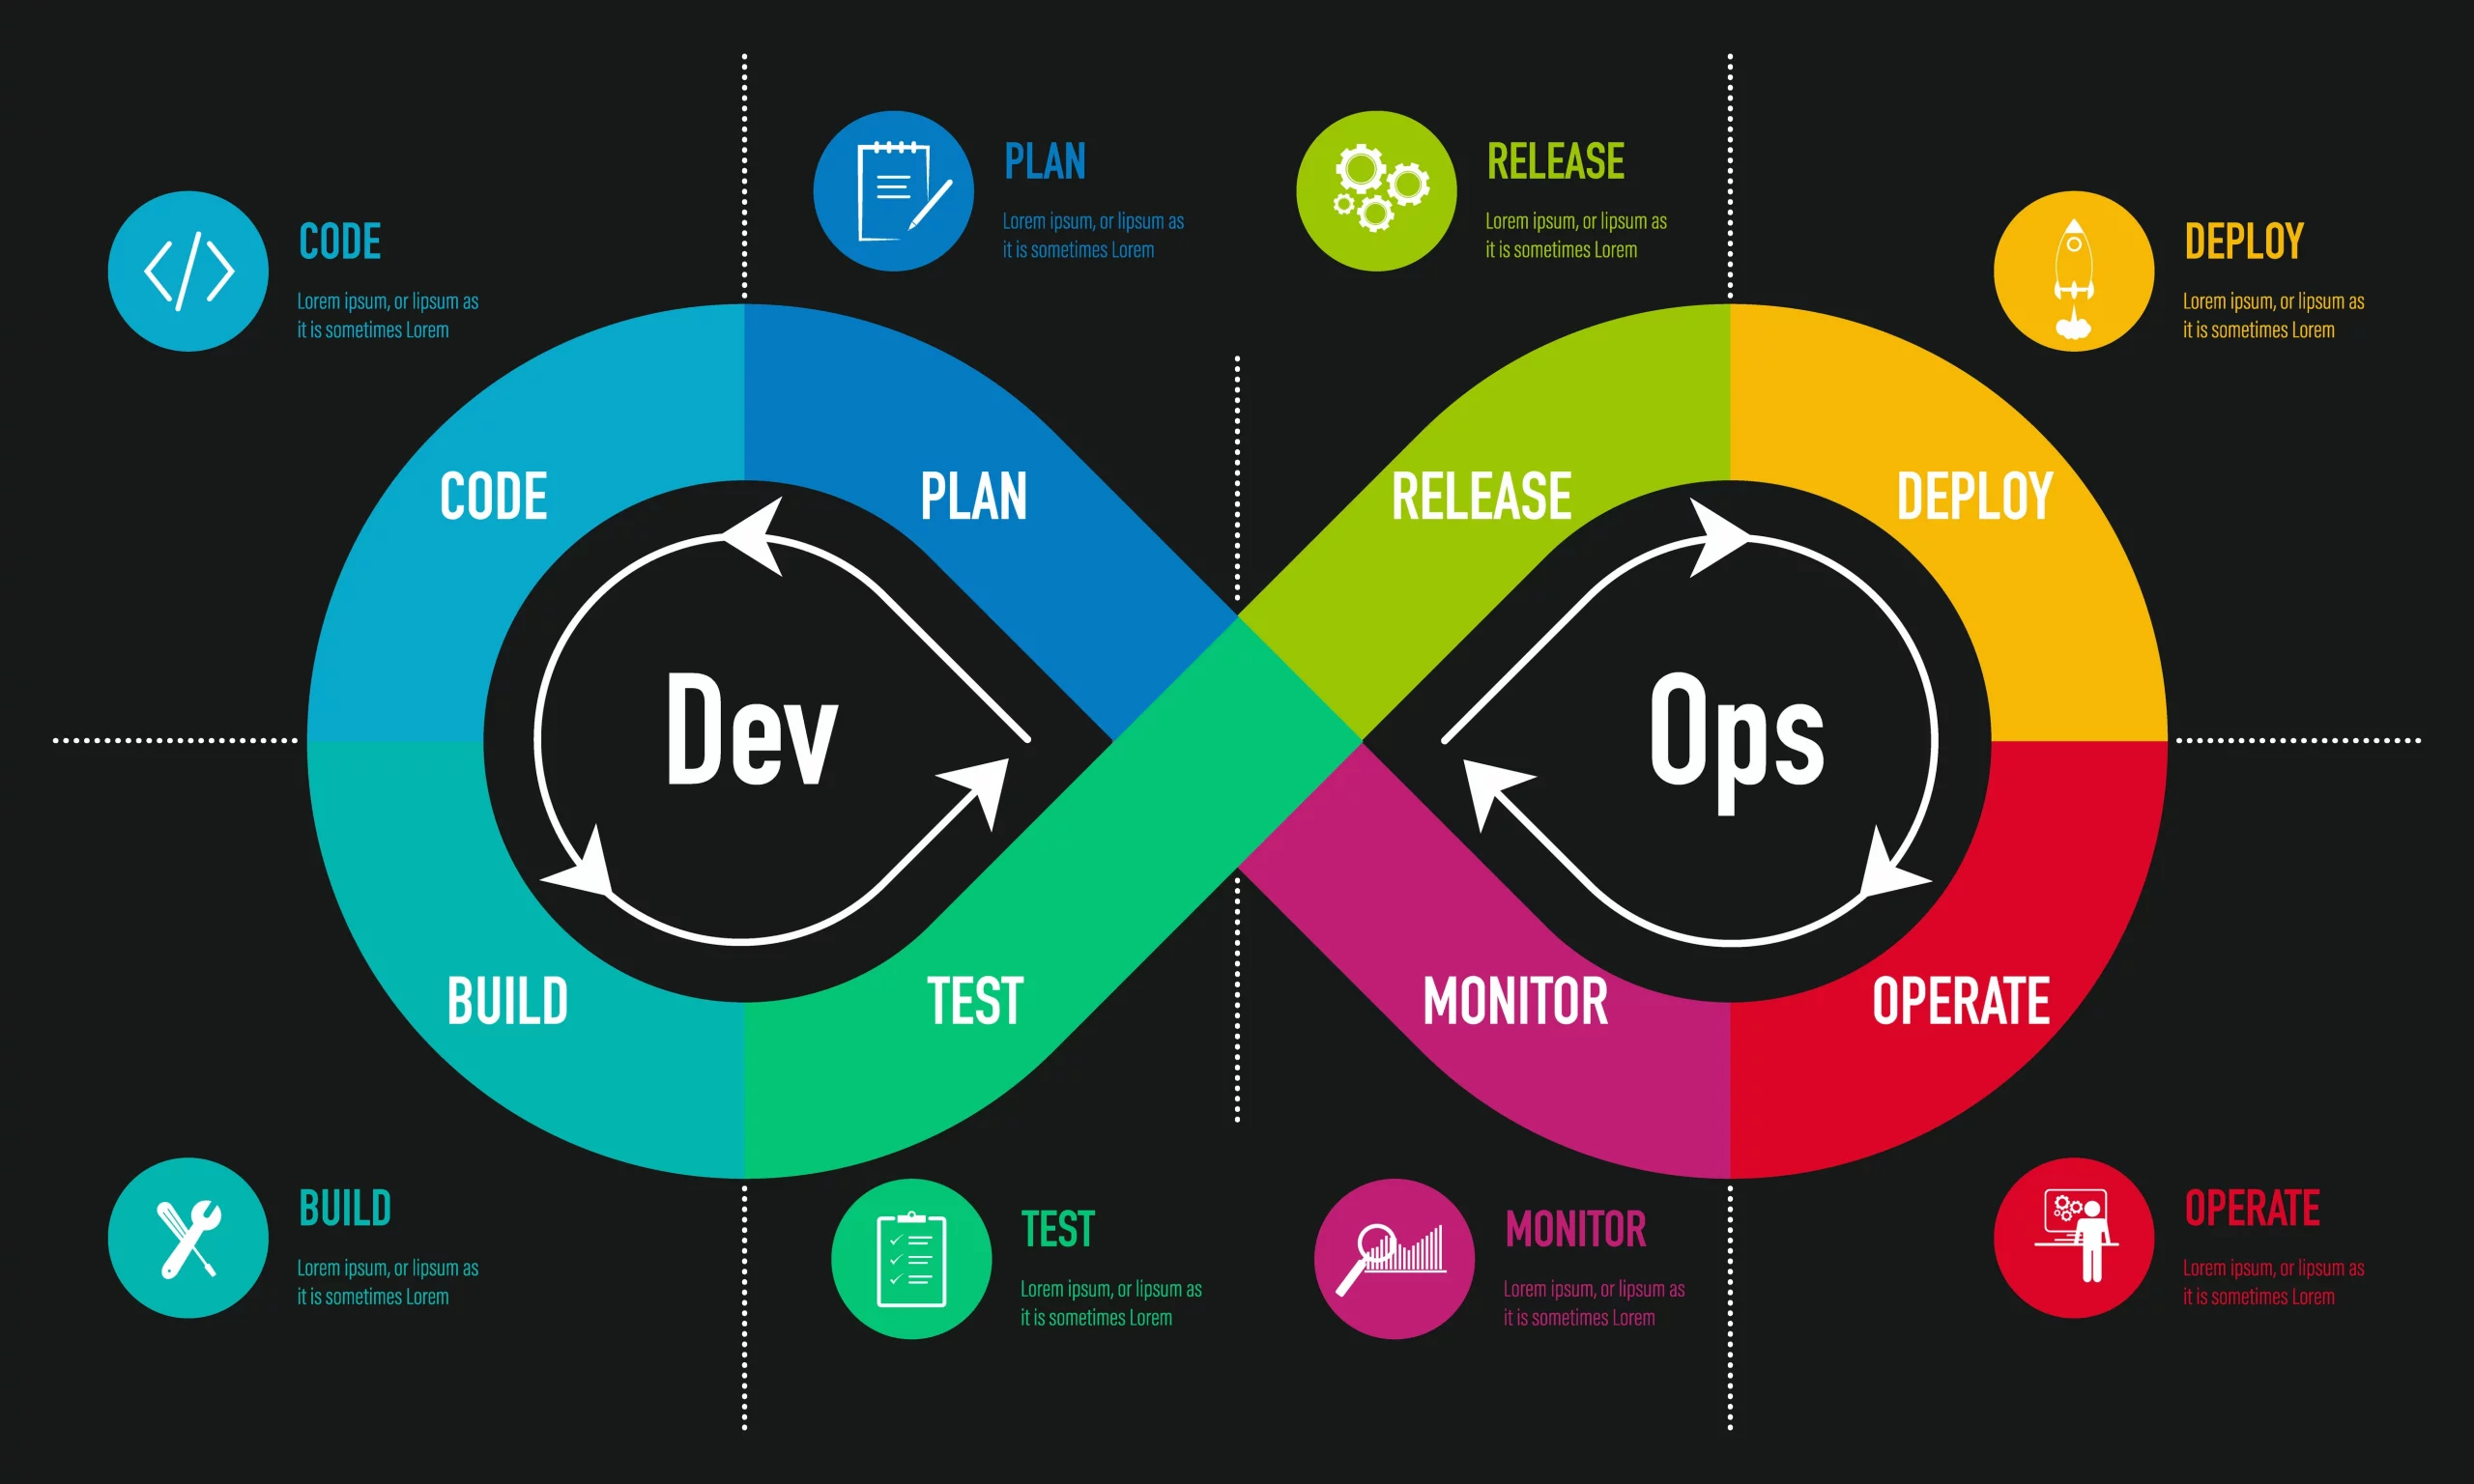
\includegraphics[scale=0.12]{images/cycle_de_deploiemnt_4.png}
\end{center}
\end{frame}

\begin{frame}{Comprendre la terminologie de Docker ? 1/2}
Avant de se lancer dans l'utilisation de Docker, il est important de comprendre la terminologie suivante :
\begin{block}{Quelques termes}
\begin{itemize}
\item[•] Image
\item[•] Conteneur
\item[•] Dockerfile 
\end{itemize}
\end{block}
\end{frame}

\begin{frame}{Comprendre la terminologie de Docker ? 2/2}
Avant de se lancer dans l'utilisation de Docker, il est important de comprendre la terminologie suivante :
\begin{block}{Quelques termes}
\begin{itemize}
\item[•] Docker compose
\item[•] Registry
\end{itemize}
\end{block}
\end{frame}

\begin{frame}

\end{frame}
\end{frame}



\end{document}
